\documentclass[11pt]{report}

\usepackage[top=1.5in, bottom=1in, left=1.5in, right=1in]{geometry}		% Set margins
\usepackage{graphicx}										% Graphics
\usepackage{subfig}											% Sub-figures
\usepackage{amssymb}										% Math formulae
\usepackage{ccicons}										% Creative Commons symbol
\usepackage[gen]{eurosym}									% Euro symbol
\usepackage{apacite}										% APA-style citations
\usepackage{fancyhdr}										% Headers
\usepackage{mdwlist}										% Compact lists
\usepackage{url}											% Fix URLs in References

\graphicspath{{./Pictures/}{./Pictures/Development/}}					% All pictures are accessed from here

\renewcommand{\bibname}{References}  							% Change "Bibliography" into "References"

\linespread{1.6}												% Double spacing


% ==== Document start ==== %

\begin{document}
\pagestyle{plain}					% No headers, just page numbers
\pagenumbering{roman}				% Roman numeral pages


% ==== Title page ==== %

\begin{titlepage}
\begin{center}

\LARGE{Using digital technology to enable new forms of\\audience participation during rock music performances}\\[0.5cm]
\large{by\\[0.5cm]
Ryan Maksymic}\\[2cm]

\includegraphics[width=0.35\textwidth]{ocadu_logo.png}\\[1.5cm]
\small
A thesis submitted to OCAD University in partial fulfillment of the\\
requirements for the degree of Master of Design in Digital Futures\\[1cm]
Toronto, Ontario, Canada, February 2014\\[1cm]
\ccLogo \hspace{0.05cm} Ryan Maksymic 2014\\[0.5cm]
This work is licensed under a Creative Commons Attribution-\\NonCommercial-ShareAlike 3.0 Unported License. To see the license go to \url{http://creativecommons.org/licenses/by-nc-sa/3.0/} or write to Creative Commons,\\171 Second Street, Suite 300, San Francisco, California 94105, USA.

\end{center}
\end{titlepage}
\clearpage
\setcounter{page}{2}


% ==== Creative Commons copyright notice ==== %

\begin{center}
\large\textbf{Copyright Notice}
\end{center}

\small
\noindent
This document is licensed under the Creative Commons Attribution-NonCommercial-ShareAlike 3.0 Unported License. http://creativecommons.org/licenses/by-nc-sa/3.0/
\\[0.3cm]
You are free:
\\
\textbf{to Share} -- to copy, distribute and transmit the work
\\
\textbf{to Remix} -- to adapt the work
\\[0.3cm]
Under the following conditions:
\\
\textbf{Attribution} -- You must attribute the work in the manner specified by the author or licensor (but not in any way that suggests that they endorse you or your use of the work).
\\
\textbf{Noncommercial} -- You may not use this work for commercial purposes.
\\
\textbf{Share Alike} -- If you alter, transform, or build upon this work, you may distribute the resulting work only under the same or similar license to this one.
\\[0.3cm]
With the understanding that:
\\
\textbf{Waiver} -- Any of the above conditions can be waived if you get permission from the copyright holder.
\\
\textbf{Public Domain} -- Where the work or any of its elements is in the public domain under applicable law, that status is in no way affected by the license.
\\
\textbf{Other Rights} -- In no way are any of the following rights affected by the license:
\begin{itemize*}
	\item Your fair dealing or fair use rights, or other applicable copyright exceptions and limitations;
	\item The author's moral rights;
	\item Rights other persons may have either in the work itself or in how the work is used, such as publicity or privacy rights.
\end{itemize*}
\textbf{Notice} -- For any reuse or distribution, you must make clear to others the license terms of this work. The best way to do this is with a link to this web page.


% ==== Author's declaration ==== %

\begin{center}
\large\textbf{Author's Declaration}
\end{center}

\normalsize
\noindent
I hereby declare that I am the sole author of this thesis. This is a true copy of the thesis, including any required final revisions, as accepted by my examiners.
\\[0.5cm]
I authorize OCAD University to lend this thesis to other institutions or individuals for the purpose of scholarly research.
\\[0.5cm]
I understand that my thesis may be made electronically available to the public.
\\[0.5cm]
I further authorize OCAD University to reproduce this thesis by photocopying or by other means, in total or in part, at the request of other institutions or individuals for the purpose of scholarly research.
\\[1cm]
Signature: \hspace{0.25cm} \makebox[7.5cm]{\hrulefill}		% Signature line


% ==== Abstract ==== %

\begin{center}
{\large\textbf{Abstract}}\\[0.5cm]
Interactive technology for an enhanced live music performance\\[0.25cm]
by\\[0.25cm]
Ryan Maksymic\\
Master of Design in Digital Futures\\
OCAD University, 2014\\[0.5cm]
\end{center}

A standard music venue has multi-coloured lights that can be controlled to set the mood of the performance; some artists, however, are not satisfied by this traditional system. Performance artists and electronic musicians have been experimenting with new technologies for years in an attempt to create a more unique and engaging stage show. Recently, many mainstream musicians have started to follow suit, incorporating clever technologies into their performances, leading to exciting experiences for their thousands of fans. Montreal-based studio Moment Factory, for instance, works with musicians like Madonna and Bon Jovi and employs special effects, mechatronics, and electronic devices to create incredible stage shows. For rock band Coldplay's most recent tour, the Xyloband - a wristband containing radio-controlled LEDs - was developed. Stadiums full of people wearing these devices lit up and blinked along with the music. It is becoming increasingly popular to enhance live events using novel technologies; however, these technologies generally lack something that I believe could greatly increase their effectiveness - interactivity.


% ==== Acknowledgements ==== %

%\begin{center}
\large\textbf{Acknowledgements}
\end{center}

\noindent
A huge thank you to my primary advisor Adam Tindale for being incredibly supportive and reliable throughout this whole process. I would also like to thank my secondary advisor Geoffrey Shea, as well as Nick Puckett, Kate Hartman, and Tom Barker for their additional support. % Martha Ladly, Marie O'Mahony
\\[0.3cm]
My thanks to Erik Grice, Blake Enemark, and especially to Christian Hansen and Molly Flood for taking the time to contribute to my research, and to Maziar Ghaderi, Jeff Royiwsky, Areen Salam, and Jackson McConnell for their help with documentation.
\\[0.3cm]
Thank you to all of my classmates and friends for always being there to celebrate and commiserate with me.
\\[0.3cm]
Lastly, I would like to thank my family for their constant support throughout my studies.

% Adam Tindale
% Geoffrey Shea
% Tom Barker
% Nick Puckett
% Martha Ladly
% Marie O?Mahony
% Erik Grice
% Blake Enemark
% Christian Hansen
% Molly Flood (check name)
% Maziar Ghaderi
% Jackson McConnell
% Areen Salam (check name)
% Jeff Royiwsky

% Classmates
% Friends
% Family


% ==== Dedication ==== %

%\vspace*{2cm}
\begin{center}
\textit{This work is dedicated to Mom.}
\end{center}


% ==== Table of contents, list of figures, list of tables ==== %

\tableofcontents
\listoffigures
\listoftables

\cleardoublepage
\pagestyle{fancy}				% Add headers with chapter titles

%\pagenumbering{gobble}			% This ensures page 1 is not numbered
\pagenumbering{arabic}


% ==== Chapters ==== %

\chapter{Introduction}

A performance is a relationship between performer and audience. Whether it is a music concert, a theatre piece, or a magic show, the performer's goal is to communicate a message. Their message could serve as a diversion from day-to-day life, or it could be a thought-provoking commentary on reality. It is always favourable, in any case, that it gets delivered as clearly as possible. Consequently, there have continually been new tools and techniques developed in order to increase the fidelity of the message. Modern sound systems can amplify a signal so it is heard for miles. Huge screens are installed to ensure all spectators have an up-close view of the performer. Venues are precisely designed to maximize audience comfort and acoustic quality. In some cases, however, it is the audience members that wish to be heard more clearly; it is the audience members that uses tools and techniques to make their messages heard. At rock and pop concerts, in addition to the customary applause and cheers, it is common to see concertgoers waving illuminated lighters and mobile phones or even holding homemade signs in the air. In a performance, the audience is as important as the performer. It is useful, then, to put more consideration into how we might deliver clearer messages from audience to performer.

\section{Motivation}

Today, musicians are more connected to their fans than ever. By leveraging services like Facebook, Twitter, and Topspin, artists can keep their followers up to date on new releases, tour dates, and other special events. Perhaps more significant is the unprecedented level of access that fans have to the musicians. Fans are talking directly to the artists, voicing their opinions on their work, providing travel tips during tours, and sharing original content inspired by them. If it is now so easy to communicate with performers via the Internet, why, then, is the communication channel at a concert still so one sided? Waving a lighter does not convey much information, and it is rare that homemade signs are actually read by the performer. Some artists have tried to develop solutions, but these have their flaws as well. Giving audience members wristbands embedded with blinking LEDs, for example, is an impressive way to expand the light show into the crowd, but it is not actually interactive, as the devices do not transmit any information from the users. Displaying audience members' Twitter posts during a show may cause some excitement, but it is also inviting them to look down at their phones, and it is not a coherent output in the context of a music performance. I believe that modern music performances can benefit from a new, reliable method of audience-to-performer communication.

% This ensures page 1 is not numbered:
%\pagenumbering{arabic}
%\setcounter{page}{2}

\section{Research Question}

The goal of this thesis project is to find the most effective communication system that will enhance a live music performance for concertgoers. This requires considering some important research questions. First of all, how might we obtain meaningful information from the audience without being a distraction to them? What information do concertgoers find meaningful? On the other hand, I am interested in what data performers might find useful. What sort of feedback could they provide that would enhance the performance for the audience? This project has a strong focus on interacting with technology. Thus, my theoretical framework will be greatly based in human-computer interaction research, ensuring that the final product is intuitive to use. With the project centred around traditional rock and pop music concerts, I am also interested in how the mind interprets this sort of music and environment. Referencing work in music psychology will help me understand why people attend these concerts and what characteristics make one performance more captivating than another. This work brings up some other topics that, while interesting, will not be addressed here. For example, while inspiration will surely be taken from other genres of music and experimental performances, the final product will be created for a standard western pop music concert. The commercial viability of the final product -- matters of distribution, pricing, etc. -- will generally not be considered.  These sorts of issues are outside the scope of this project.

\section{Overview}

To begin, I will examine related academic and professional work. Next, the methods and results of my primary research will be discussed. My prototyping process will then be explained, followed by an analysis of the results from the user testing. Last is a discussion on the outcome of the project and possible future directions.

\chapter{Background}



\chapter{Research Question}

This chapter will provide an in-depth examination of my research question. Through referencing the existing research outlined in the previous section, I will justify the need for my work. I will then explain the steps I will be taking to address this question.

\section{Research Question}

% Questions:
How can technology best be used to add participatory elements to traditionally presentational rock and pop concerts?
% * How do audiences want to participate? How do performers want audiences to participate?
% * Input: How can data best be captured from the audience?
% * Output: What can the audience interact with that will enhance the performance but not distract the audience or performer?
% * Feedback: What kind of feedback will be informative/useful without being distracting?
% * What's the threshold where a performance can no longer be social? What's the ratio where participation can be sustained?
% * Many maintain that music is inherently social, so is anyone explicitly calling out presentational performances as unnatural? Should I do this?
% * Small shows are much, much cheaper than arena shows, and they offer much more personal experience. So why are we paying \$500 for arena shows? Are we getting our money's worth? Does the spectacle make up for the separation?

% Justification: 
% * Interactivity at rock concerts has not been thoroughly examined, despite the fact that people are making these systems in the real world
% * The performer's perspective is rarely investigated, and this is just as important as the audience's perspective
% * The impact of social media on live performance has not been analyzed in this way


\section{Hypothesis}

% Background:
% Auslander, 1999: Communities are formed based on how the audience interacts, with no dependence on the spectacle at hand
% Turino, 2008:
% * Artists can shift between participatory and presentational performance
% * Different roles of different difficult allow for everyone to feel welcome and achieve flow. "Core" and "elaboration" roles cater to advanced and non-advanced performers respectively.
% * Open form: Basic motives repeated over and over. Easy for newcomers to join in. "Security in constancy." Can facilitate flow.
% * Hall: Repetition can increase intensity. Synchronicity comforts people.
% * Wide tuning, loud volumes, and overlapping textures provide a ``cloaking function'' that makes people more comfortable participating
% * Virtuosic solos are not common
% * Some participatory performances are sequential -- everyone gets a turn (e.g. Karaoke)


% Hypotheses:
% * 


\section{Approach}

% Methods:
% * Questionnaire and interviews (User-centred design; Ethnography)
% * Prototyping and user testing (User-centred design)
% * Real-world testing (Action research, participative objective observation; Ethnography)

\chapter{Preliminary Research}

One of my first goals was to get a sense of modern concertgoers' and performers' feelings about participatory performances and interactive technology. I sent out a brief online survey for music fans that helped me to understand how they generally responded to these topics. Interviews were also conducted with multiple musicians to shed light on their perspectives.

\section{Audiences}

% Explain the content of the survey:
An online survey was created in order to obtain a sample of modern music fans' opinions on interactive performances. The survey was completed by ninety-nine participants recruited via social media. The first few questions informed me of what type of concertgoer each participant was -- asking their favourite genre, the size of the venues they frequent, and how often they attend live music performances. I also asked how often the participants communicate directly with musicians through their social media presences. Next, the survey focused on concert behaviours. Participants were asked in which actions they typically partake at live music performances; choices included applauding, headbanging, and holding up lighters. They were asked how they might like to interact with their favourite performer and what sort of message they would send them if they could. I asked for their thoughts on getting involved in performances, bringing new technologies into concert settings, and interacting with musicians using social media services. (For complete results, see Appendix X.)

% Present the direct results:
The results were not shocking but certainly informative. Most participants favoured rock music or some variation (``indie," ``alternative"); the majority attended multiple concerts per year -- some even on a weekly basis; and most usually went to shows at small- to medium-sized venues. The majority of participants claimed to communicate with artists through social media either sometimes or regularly, though a sizeable amount indicated they never do this. The most popular concert actions were applauding, singing along with the performer, clapping or stomping to the beat, dancing, jumping up and down, and chanting words or phrases along with the other audience members. When asked how they might want to interact with a performance, many said they would like to choose the songs that are played, while much fewer expressed interest in manipulating visuals and contributing to the music; around one quarter of participants stated they did not have interest in directly influencing a live music performance at all. Given the opportunity to communicate with their favourite performer, most participants responded with praise or appreciation (``Thank you," ``I love you!"). Other messages included song requests and suggestions like, ``Don't bury the vocals," or ``More rock, less talk!" The majority of participants indicated that they enjoy when performers ask them to participate in a performance -- clapping or singing along or call and response, for example. Lastly, the majority also said they were excited by the idea of bringing new technologies into a live music setting.

% Present the results of the in-depth analysis:
Upon further analysis of the responses, some correlations were uncovered. There are clear relationships between show-going frequency, venue size, and interest in interaction and technology. Participants attending shows more frequently are more likely to visit smaller venues. This group also expressed the most interest in being involved in performances; they are more inclined to interact with their favourite artists via social media; and they are more welcoming to the idea of unfamiliar technology in a concert setting. The opposite, thus, can also be said: participants who go to fewer shows tend to go to larger venues, are more likely to refrain from participating in shows, are less likely to contact artists through social media, and are less interested in new technologies.

% Conclusions:
A few general conclusions can be made from these results that are particularly relevant to my research question. It is encouraging to confirm that most participants are not quietly standing still at live performances; they are cheering, moving, and singing along. A surprising find was that, given the chance to say anything to their favourite artist on stage, most participants would choose simple messages of praise or thanks -- something ostensibly achieved already by applauding. Also intriguing was the relative lack of interest in influencing lights and visualizations. Instead, the majority of participants showed great interest in choosing the set list for the performance. Regardless, it is clear that most respondents have little to no reservations about being directly involved in a show and doing so with new technologies. Seemingly, this willingness to interact is more common in those who frequently attend performances at smaller venues. Perhaps, then, artists that play to smaller crowds and can offer more direct interactions both on and off stage have fan bases that are more willing to experiment with new interactions.


\section{Performers}

% Explain the interview participants and questions:
With a broad overview of audience attitudes, the next step was to speak directly with actual performers and see how their opinions compared. Four musicians -- Christian, Erik, Blake, and Oliver -- were interviewed, all members of different bands that perform some variation of rock or pop music, with typical audience sizes ranging from fifty to five hundred people. After briefly establishing their history as performers, I asked each about how they like to interact with their fans. The musicians were shown video of some of my case study subjects (including Xylobands, Wham City Lights, Kasabian), and I asked for their reactions and general thoughts on technology-enabled performances. Lastly, the artists were asked how they might want to incorporate participatory technologies into their own shows.

% Christian:
Christian is the frontman for a Toronto-based new wave group that has been active for several years. He comes from a theatre background but has been playing in bands since he was fourteen. Christian was performing acoustic music during his post-secondary degree, but he was growing increasingly fond of dance music, and he eventually formed a duo that made use of computer software to play danceable pop music.


\chapter{Development}

%This section describes the chronology of this project's various prototypes. The successes and failures are described, giving the overall story of how I arrived at my final product.

\section{First Phase}

\subsection{Objectives}

The goal of the first prototype was to simply demonstrate how multiple users might interact with a performance using handheld devices. To realize this, I used Wii video game controllers and the Max visual programming software. The final product was to be a VJ system where one user (the ``performer") could manipulate looping video clips using a Wii controller and multiple ``audience members" could contribute to this manipulation to a lesser degree with their own individual controllers.

\subsection{Prototyping}

My first milestone in this prototype was having a single Wii controller communicate with my computer. Using a program called OSCulator, I was able to read movement and button-push data sent via Bluetooth (see Figure \ref{prototyping1}). From here, the data is sent to a simple Max program (called a ``patcher") that I created. The patcher reads various movement data from the controller and visualizes them as different motions that a typical concertgoer might perform. The motions are: giving a ``thumbs up" or ``thumbs down", swaying arms from side to side, clapping, or doing ``the wave," as shown in Figure \ref{prototyping2}. Visual feedback is provided in the form of illuminated LED objects and moving sliders.

\begin{figure}[t]
	\centering

	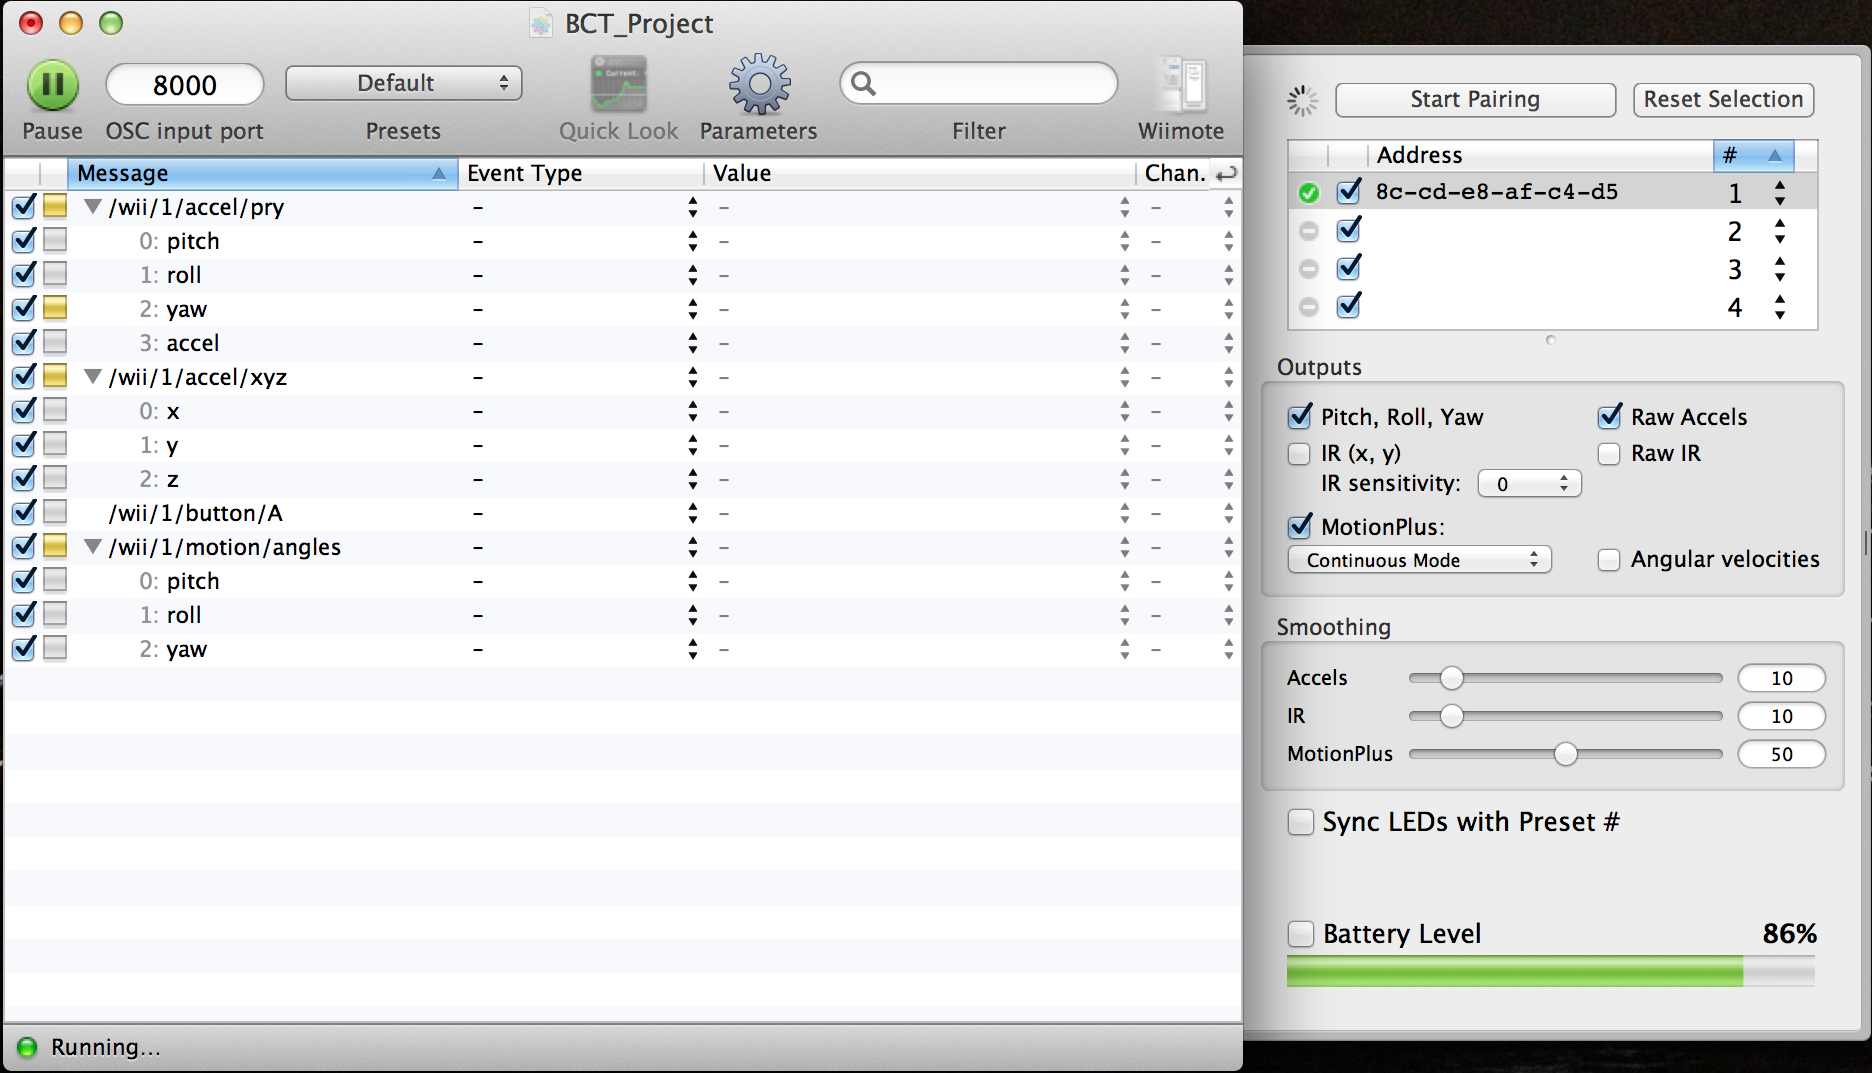
\includegraphics[height=0.3\textwidth]{osculator_1.png}
	\caption{OSCulator software receiving data from one Wii controller}

	\label{prototyping1}
\end{figure}

\begin{figure}[t]
	\centering

	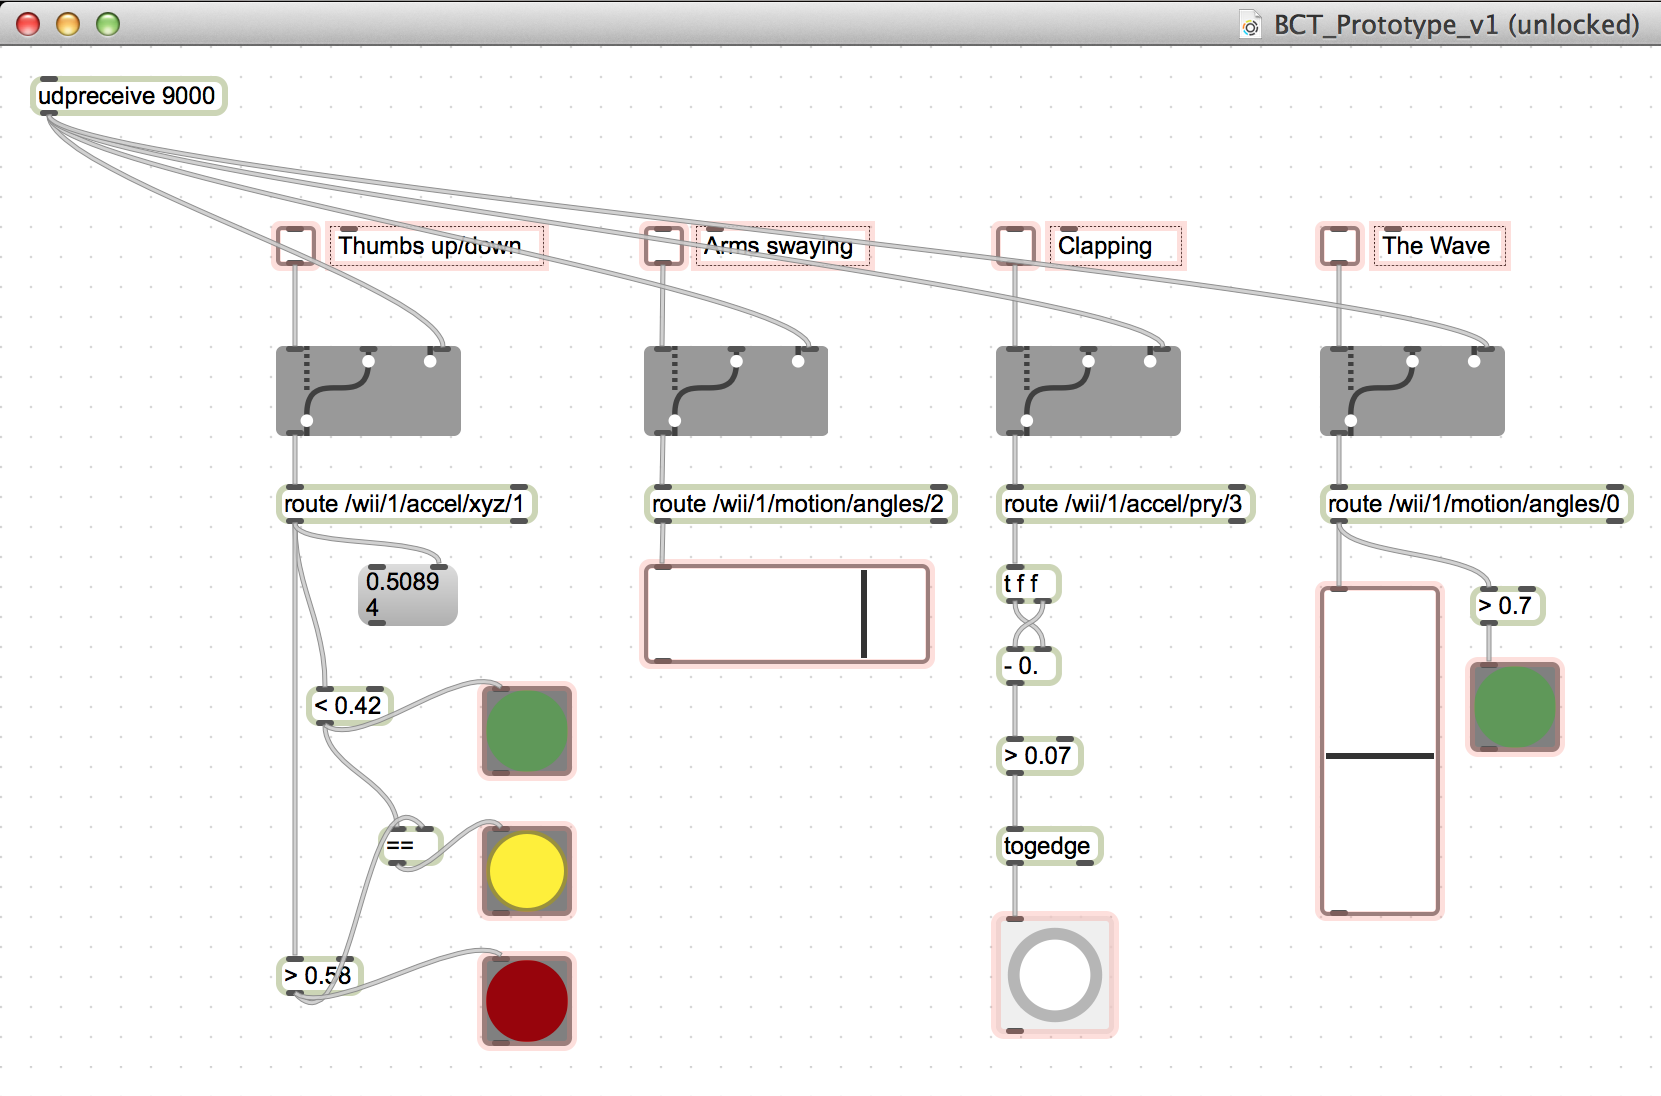
\includegraphics[height=0.3\textwidth]{wiimote_audience.png}
	\caption{First Max patcher}

	\label{prototyping2}
\end{figure}

My second notable achievement was testing the limit of how many Wii controllers would be able to connect to my computer using the current setup. Since my thesis aims to give every member of an audience a new way to communicate, this number would ideally be limitless. The OSCulator software, unfortunately, could only connect to a maximum of seven controllers. However, for the purposes of this prototype, this number is acceptable. To test this, I created a Max patcher to display data from seven Wii controllers. I synced all seven controllers with OSCulator with no issues, and the program worked as expected (see Figure \ref{prototyping3}).

\begin{figure}[t]
	\centering

	\subfloat[Wii controllers]{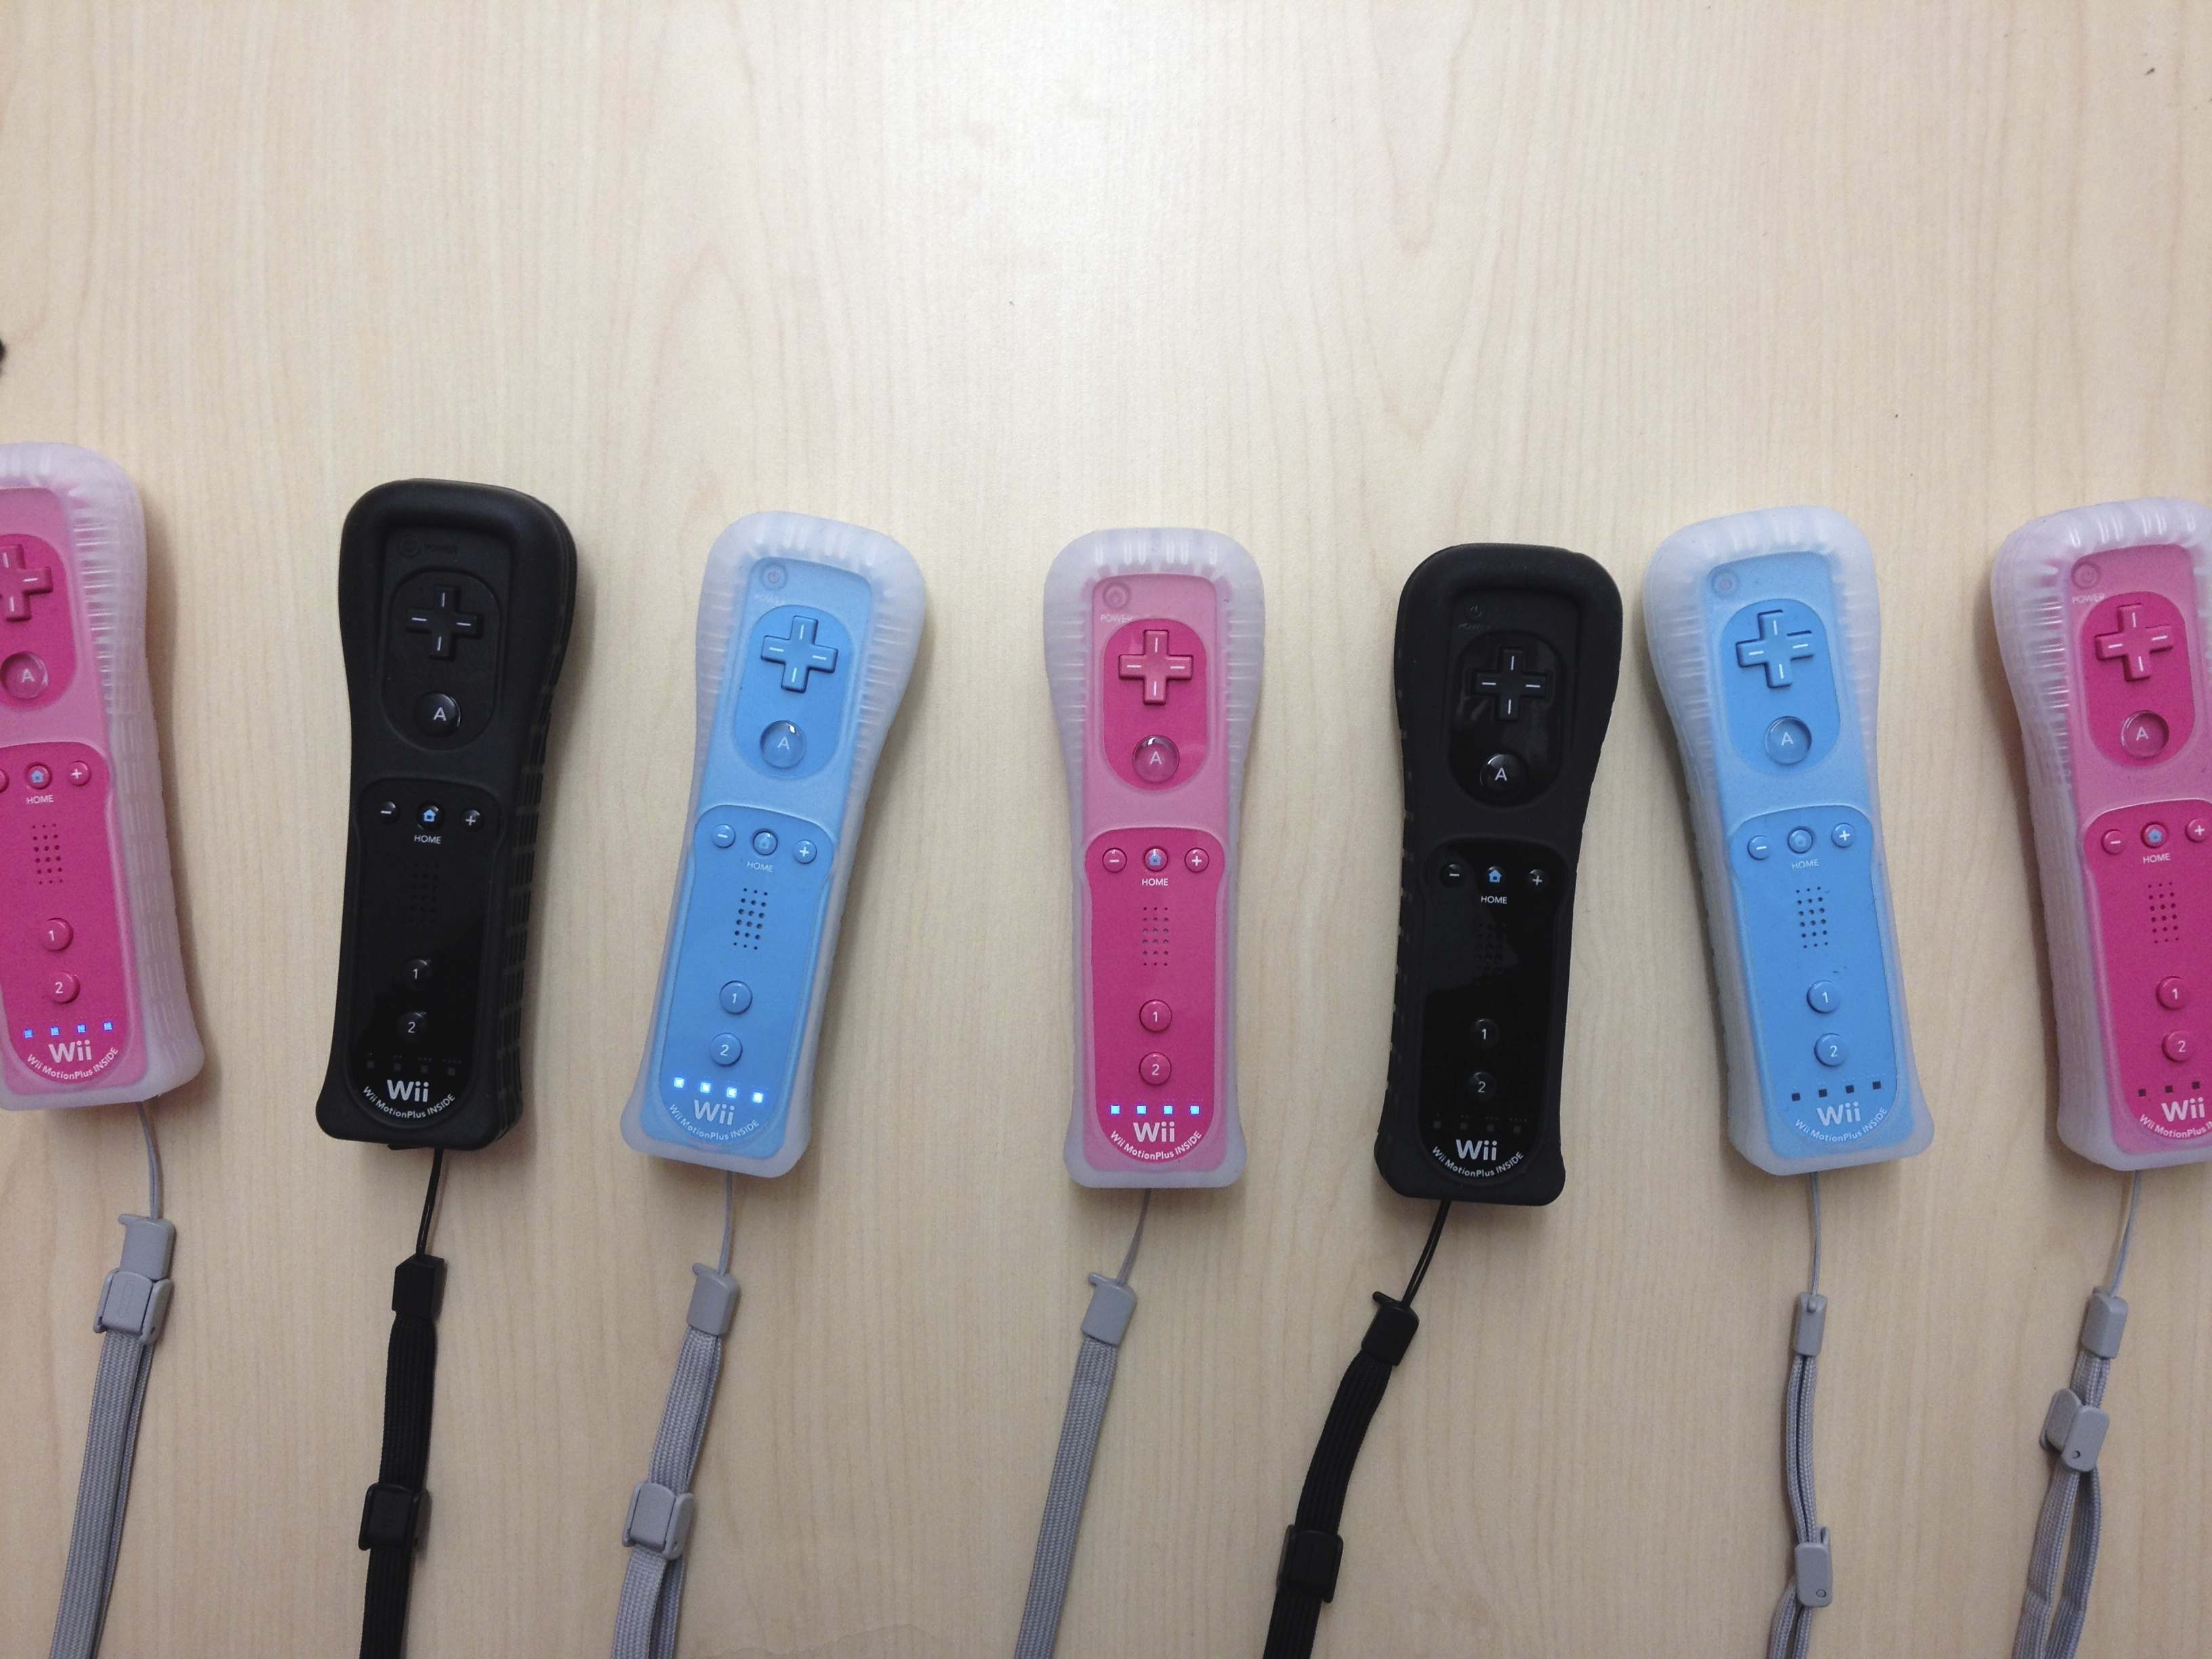
\includegraphics[height=0.32\textwidth]{wiimotes.jpg}}
	\hspace{0.1cm}
	\subfloat[Max patcher]{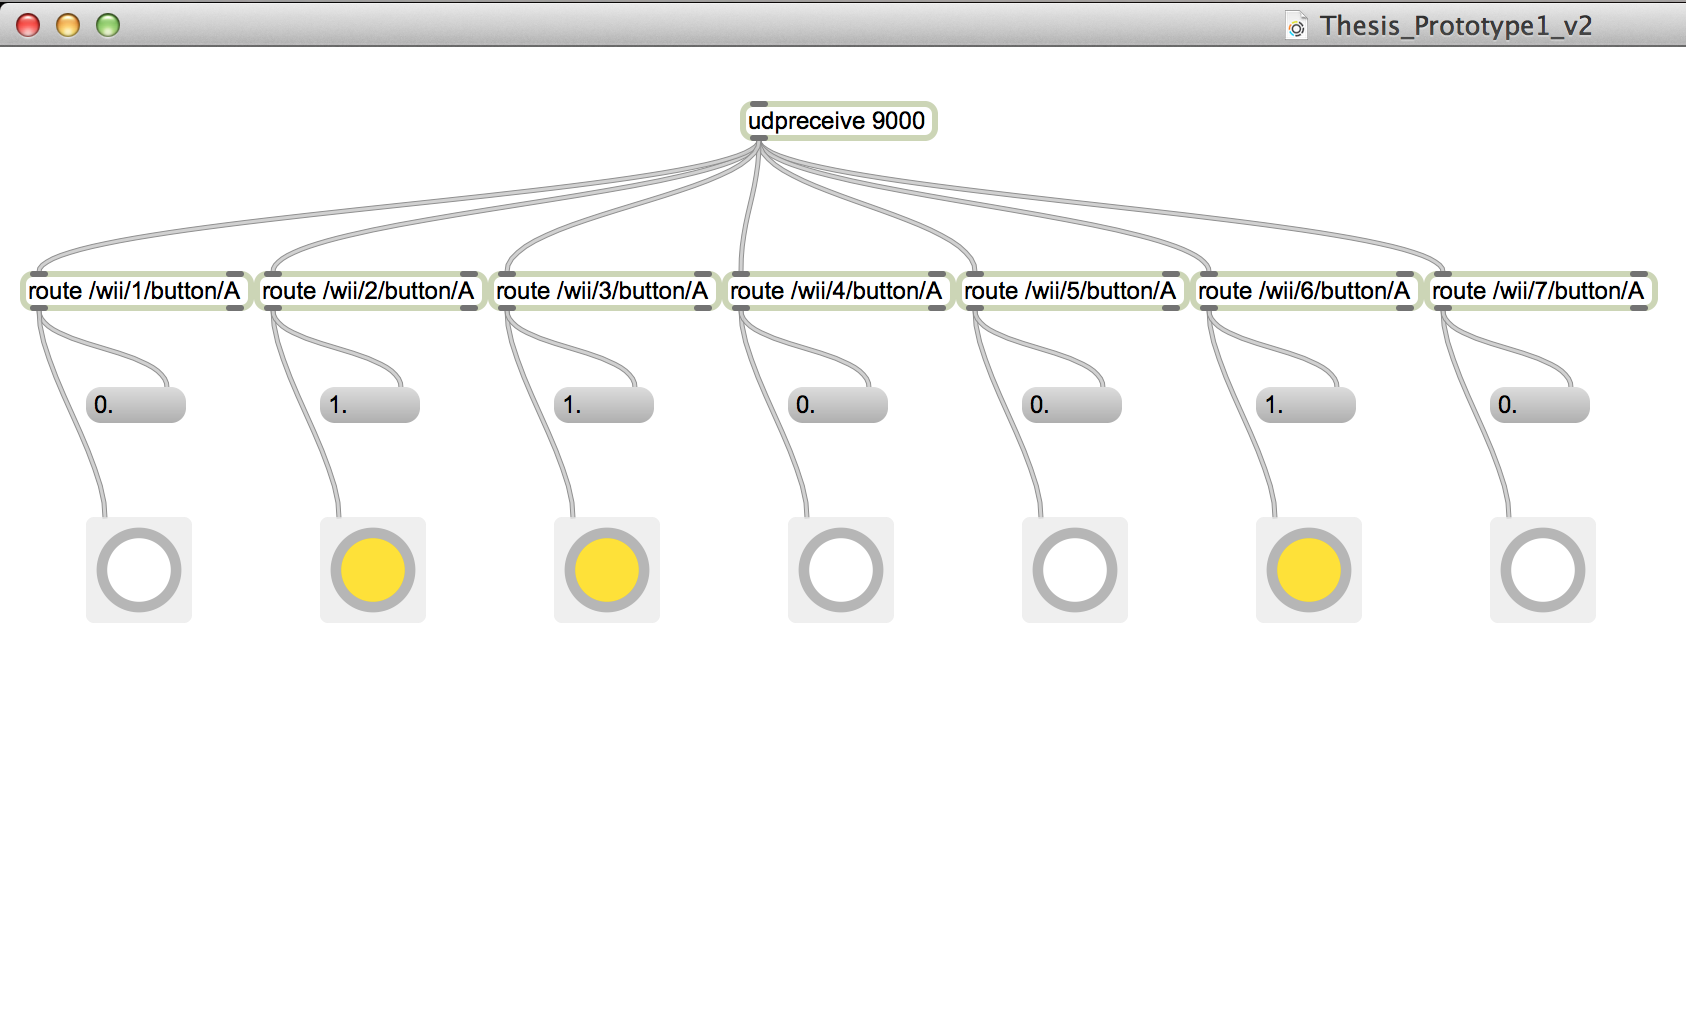
\includegraphics[height=0.32\textwidth]{multi_wii.png}}
	\caption{Testing simultaneous input from seven Wii controllers}

	\label{prototyping3}
\end{figure}

The next goal was to have multiple Wii controllers collaboratively manipulating a video in some way. I decided to create a patcher where users could ``vote" for how to control the video. In this case, I fed two video loops -- one monochrome clip of one person dancing and one colourful clip of multiple people dancing -- into a crossfader object. By pressing and holding the Left or Right buttons on their controllers, users can vote on which clip dominates the screen. In an effort to experiment with multiple motion data, I also incorporated a mechanism that lets users make their votes count double by shaking their controllers. Lastly, I packaged all of these programming objects into a ``sub-patcher," making the program more modular and readable. Figure \ref{prototyping4} shows the patcher running with three users.

\begin{figure}[t]
	\centering

	\subfloat[Main patcher]{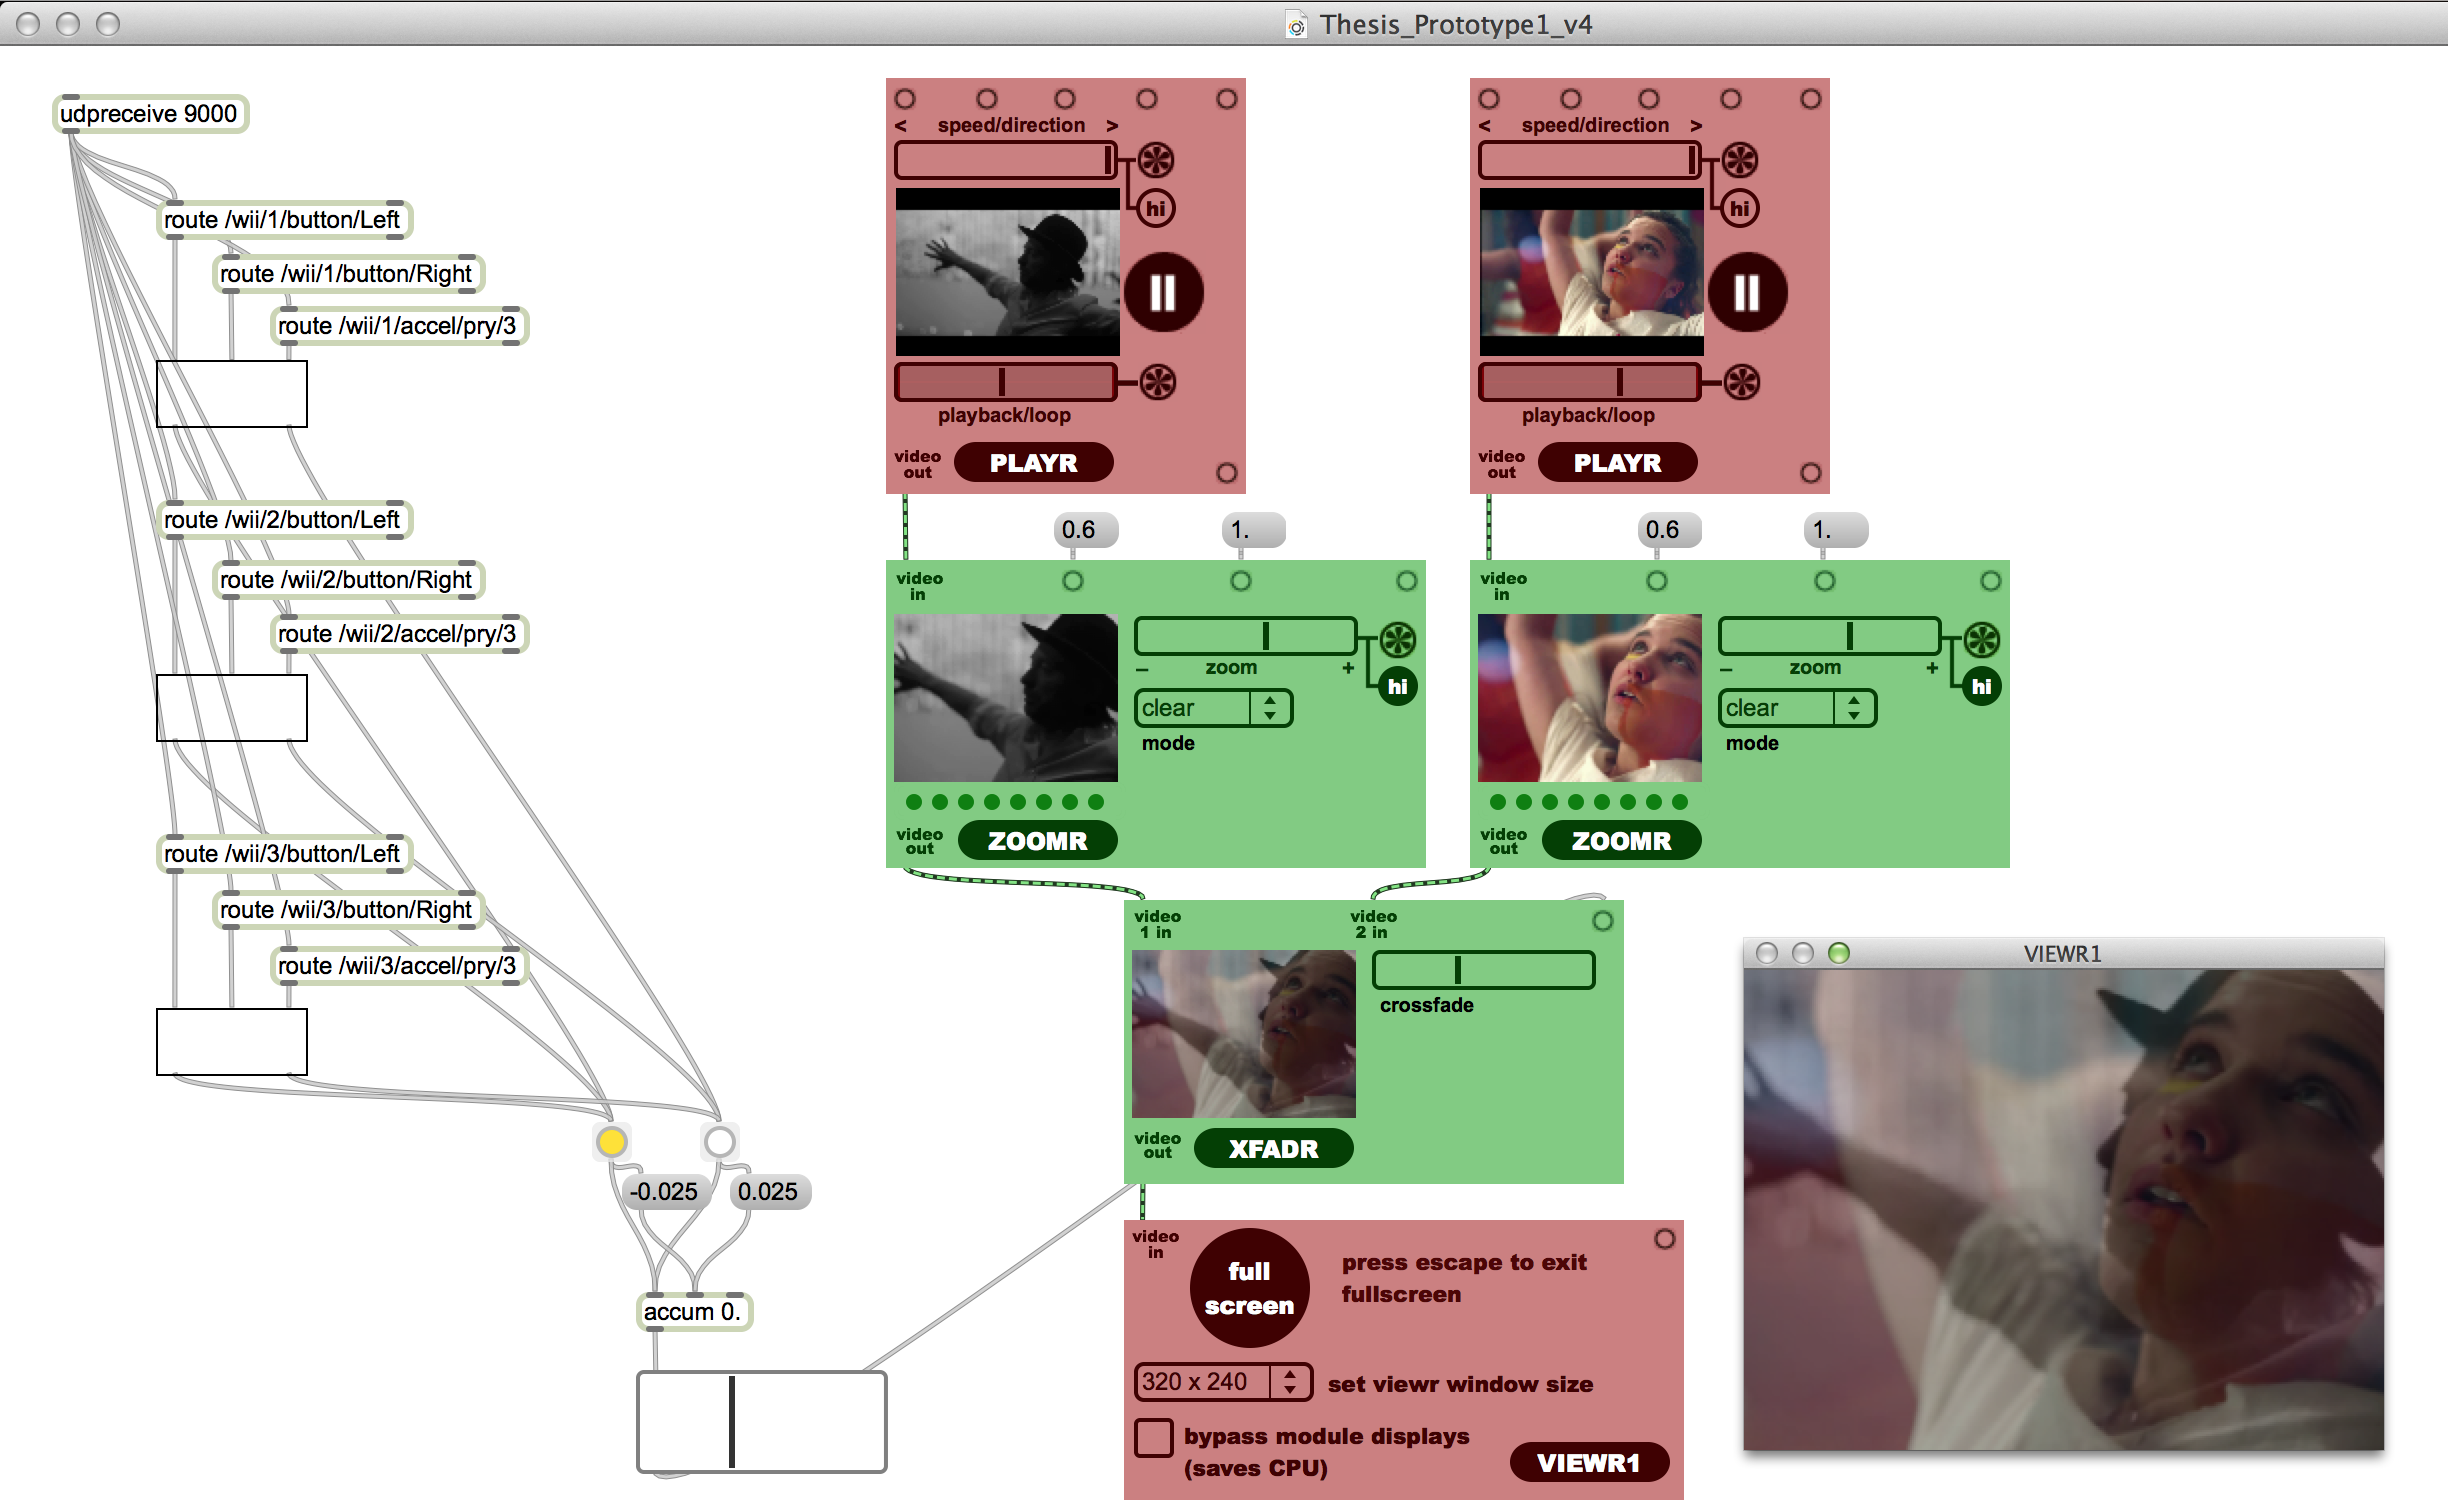
\includegraphics[height=0.3\textwidth]{threewii_voting.png}}
	\hspace{1cm}
	\subfloat[Sub-patcher]{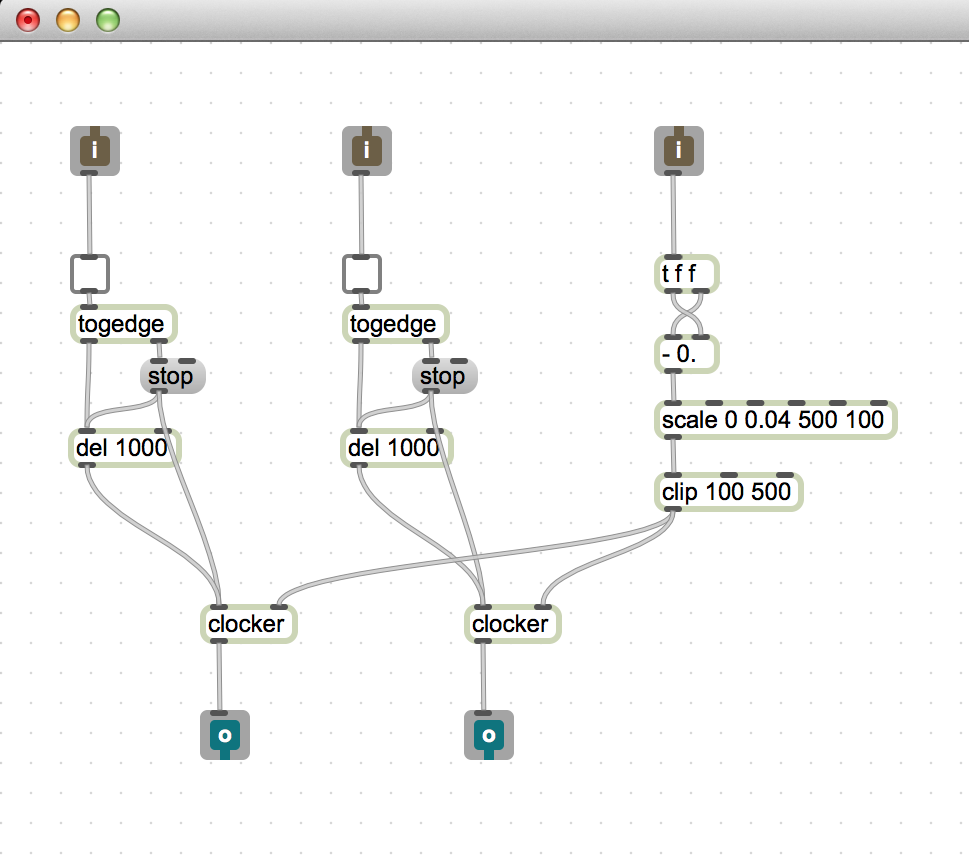
\includegraphics[height=0.3\textwidth]{threewii_voting_sub.png}}
	\caption{Video effect voting system with three users}

	\label{prototyping4}
\end{figure}

My next task was to create the VJ program for the performer in my scenario. I spent a lot of time experimenting with video effects in Max. I selected four effects objects that would allow the performer to rotate the image, control pixelation, enable a motion blur effect, and crossfade between two video loops. These are controlled by rotating the Wii controller, increasing the incline of the controller, pressing and holding the A button, and pressing the Left and Right buttons, respectively. An important part of programming this patcher was mapping the data from the controller to the effects controls. Values had to be carefully scaled and clipped in order for the user's movements to translate naturally to the effect they control. The patcher is pictured in Figure \ref{prototyping5}.

\begin{figure}[t]
	\centering

	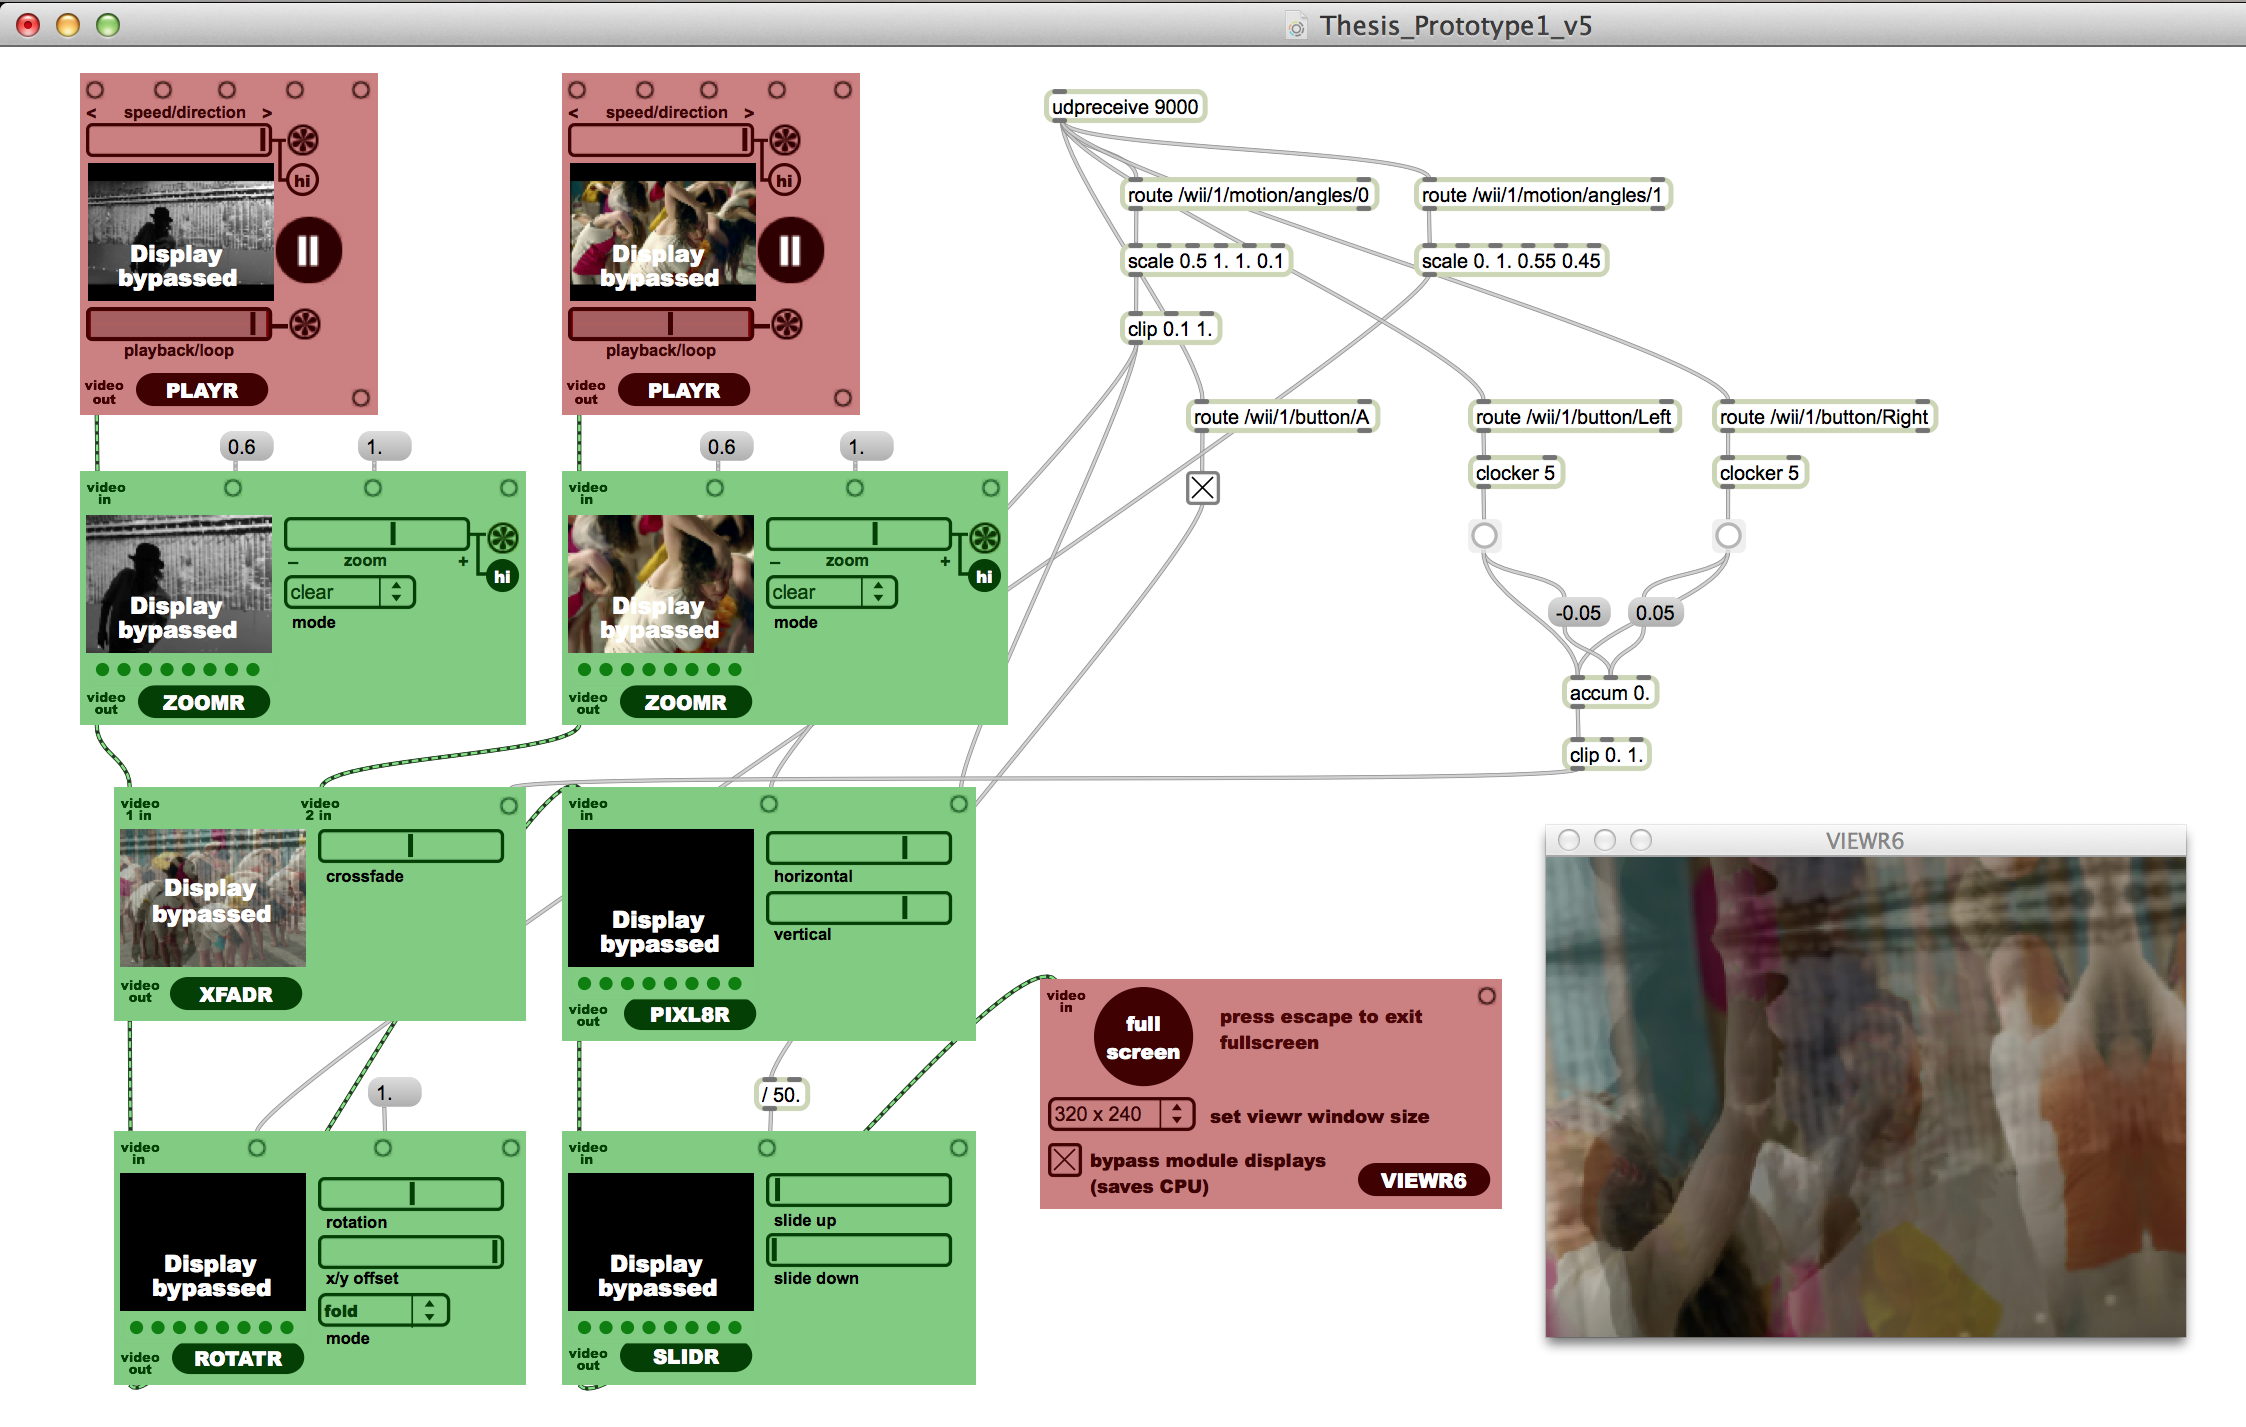
\includegraphics[height=0.3\textwidth]{wii_vj.png}
	\caption{Wii controller VJ system}

	\label{prototyping5}
\end{figure}

The results of the last two victories were finally combined to create my audience-performer interaction system (see Figure \ref{prototyping6}). Here, one user has the VJ controls described in the previous section. The audience voting system, however, is also implemented, allowing the other users to collaboratively control the crossfading of the two clips. Thus, as the performer simultaneously manipulates the two loops, the audience can decide which of them dominates the screen. Additionally, using the controller's B button, the performer has the ability to ``mute" the audience if their input is no longer desired. This stage required development of more sub-patchers to condense and modularize the program.

\begin{figure}[t]
	\centering

	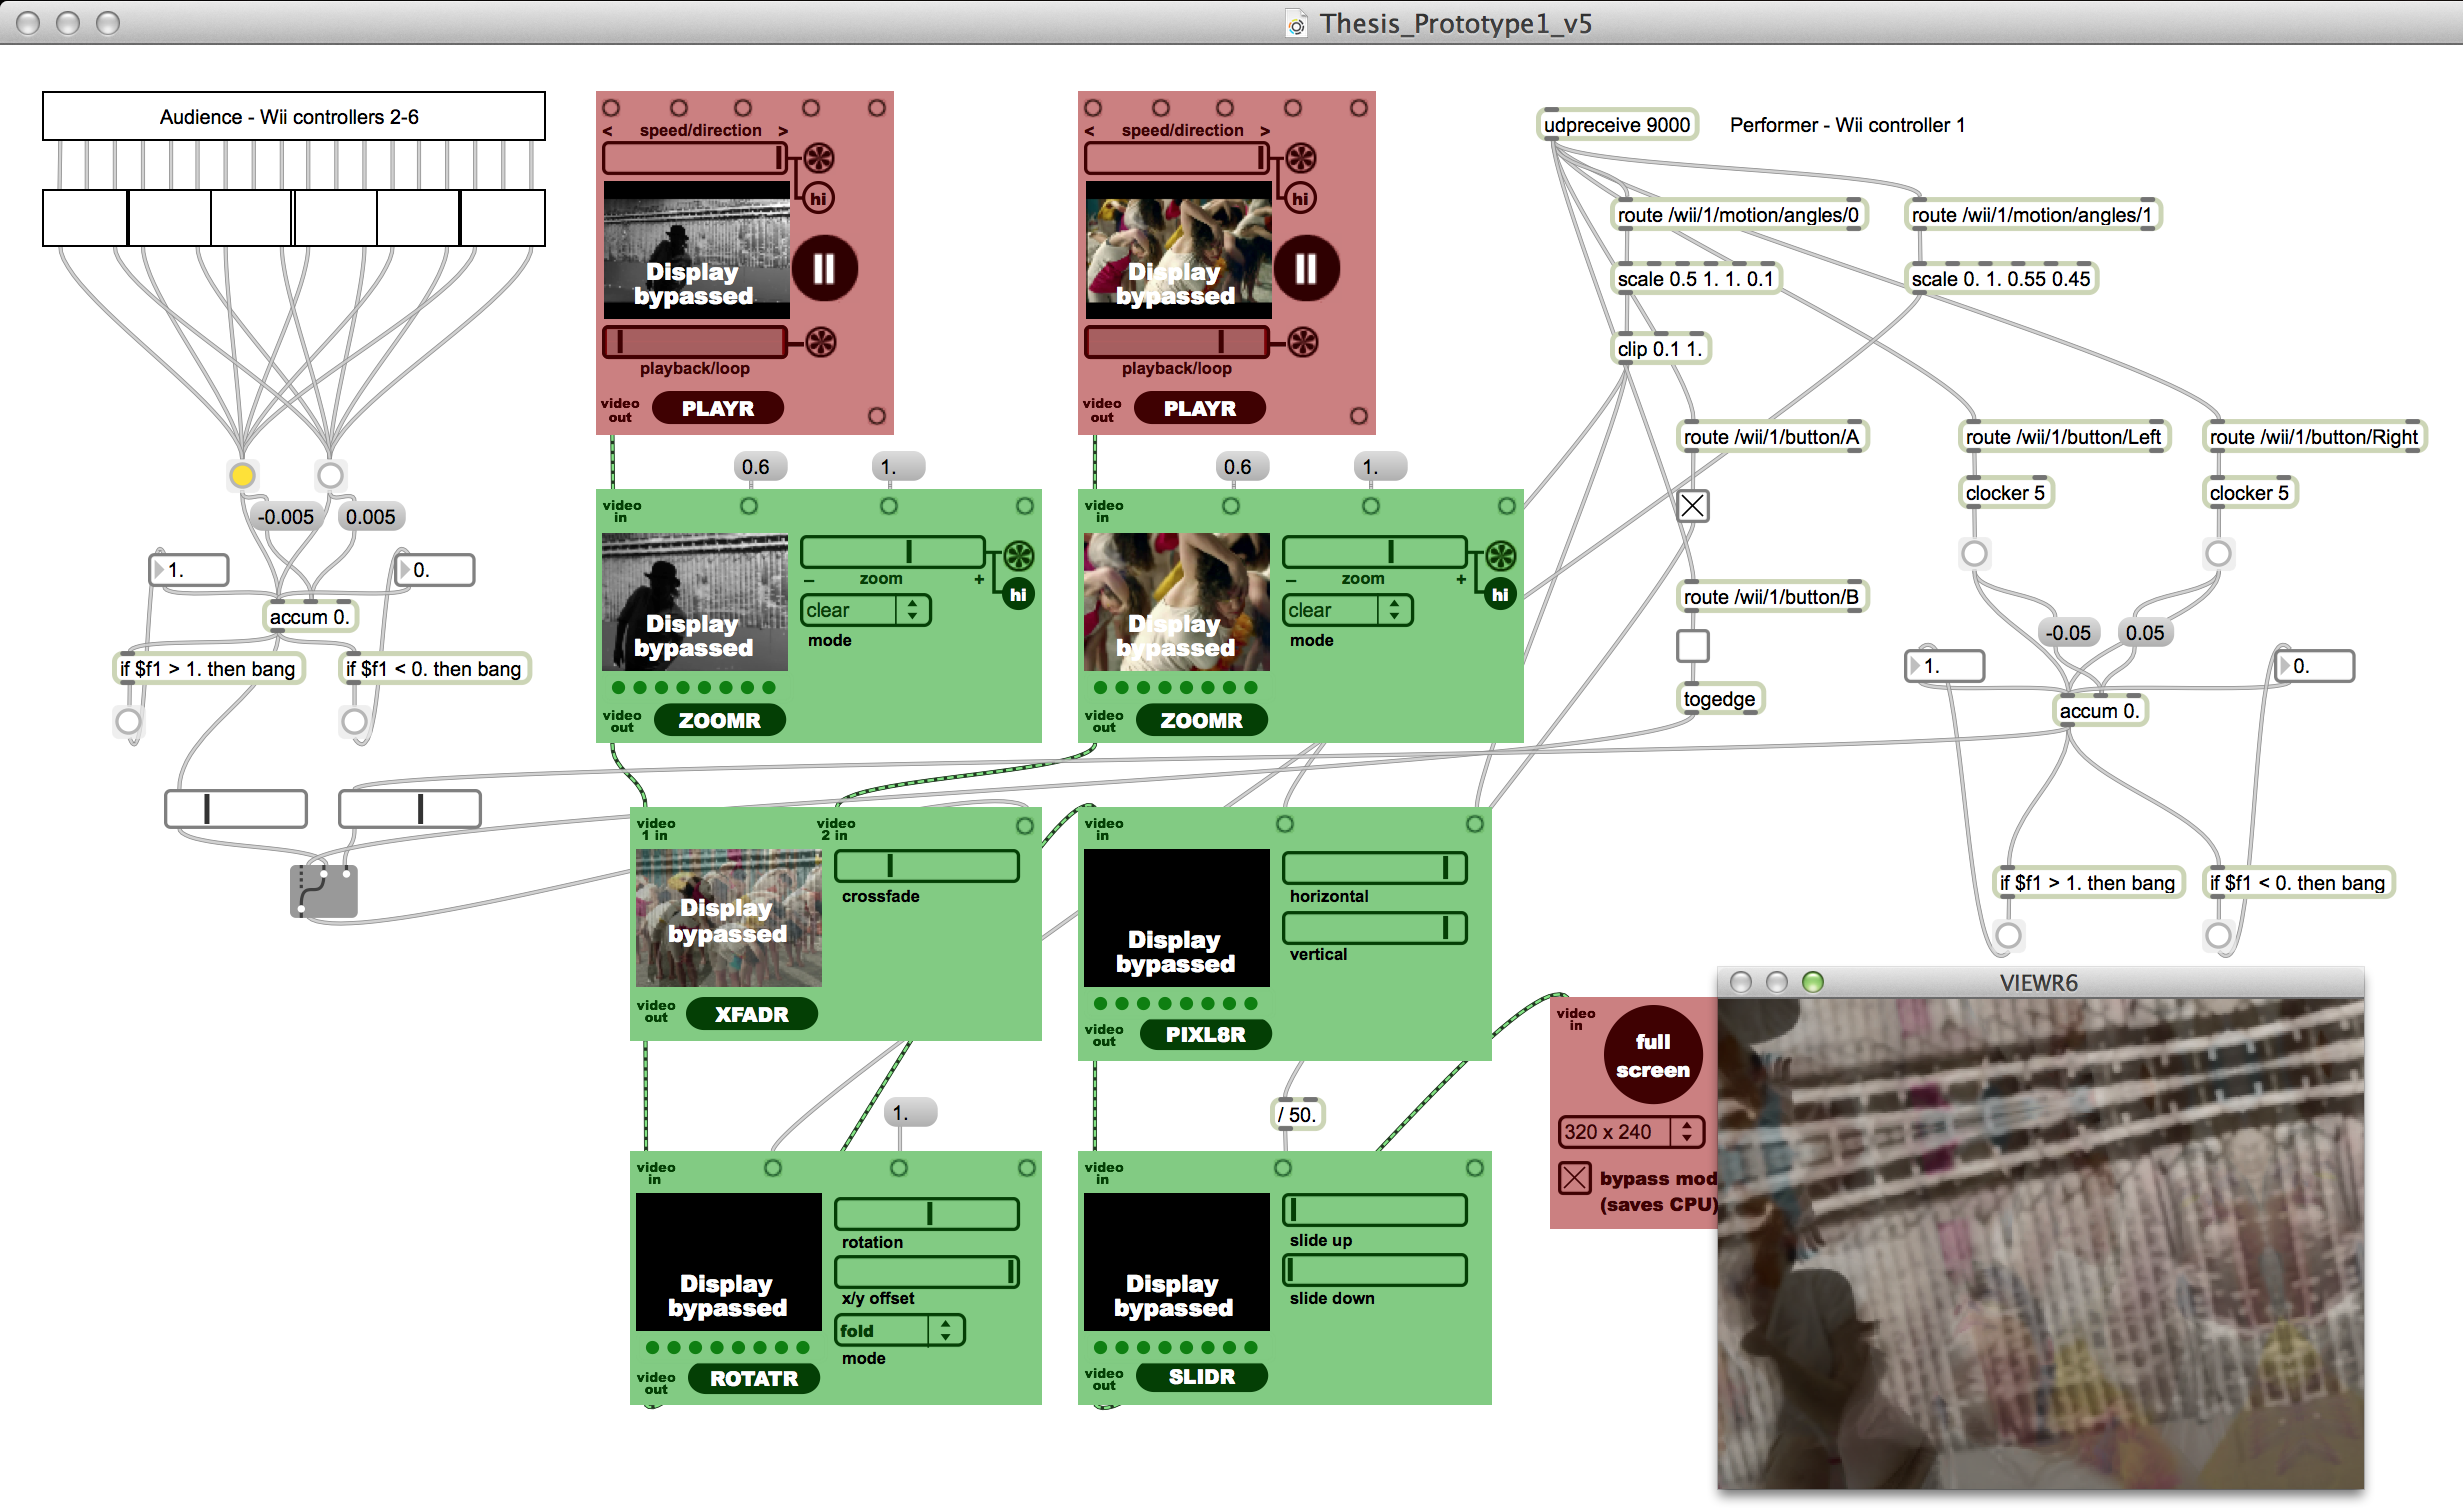
\includegraphics[height=0.3\textwidth]{vj_and_audience.png}
	\caption{Audience-performer interaction system}

	\label{prototyping6}
\end{figure}

\subsection{User Testing}

\section{Second Phase}

\subsection{Objectives}

\subsection{Prototyping}

\subsection{User Testing}

\chapter{Implementation}

\section{Production}

\section{Event}

\section{Reflection}

\chapter{Conclusion}

\section{Discussion}

\section{Future Directions}

% A dynamic system that allows for performance-long audience participation but changes the rules periodically to maintain their interest

% Use colour to indicate associations or rule changes

% User testing can involve those present but not participating. How was the experience changed for them?

\section{Conclusion}


% ==== Bibliography ==== %

\nocite{*}						% Cite everything in the BIB file
\clearpage
\bibliographystyle{apacite}
\bibliography{Thesis}


% ==== Appendices ==== %

%\chapter{Research Ethics Board Materials}


\end{document}